%!TEX root = groundunitbriefing.tex

% LTeX: enabled=true

\clearpage
\twocolumn[
    \section{Ground Targets}
]

A ground \emph{target} is a unit of infrastructure such as a bridge and a building.

\begin{figure}[ht]
    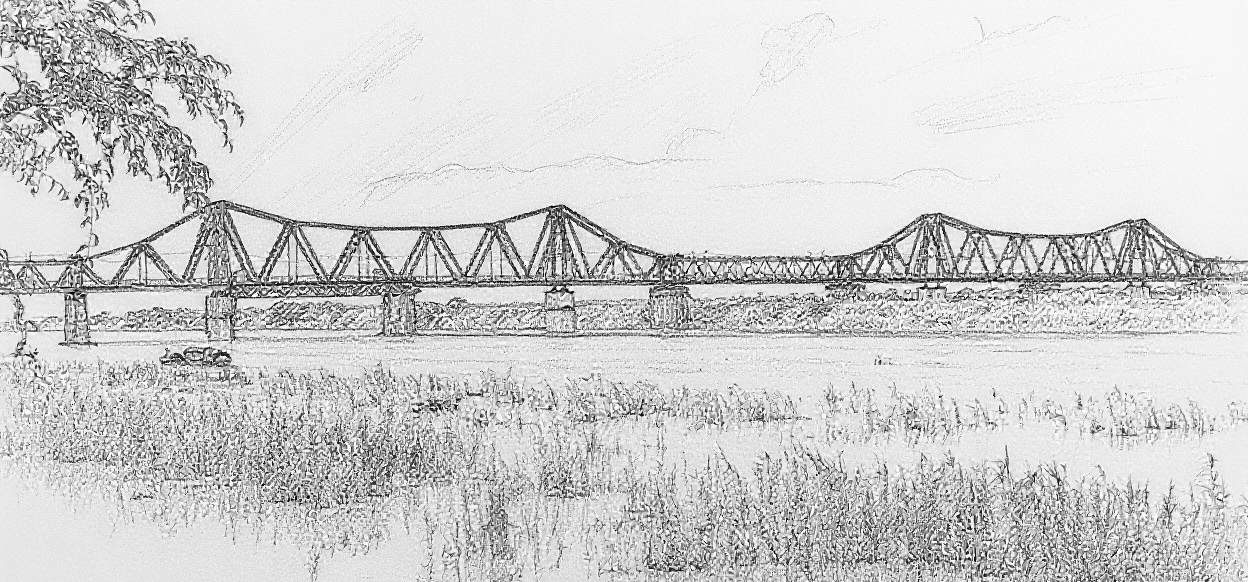
\includegraphics[width=\linewidth]{photos/paul-doumer-bridge.jpg}
\end{figure}

\subsection{Properties and Representation}

Ground targets are listed with their properties in Table~\ref{table:ground-targets}.

All ground targets have these properties:
\begin{itemize}
    \item defense strength;
    \item defense strength and target class;
    \item sighting range in hexes; and
    \item the VPs awarded for 3D/2D/D damage.
\end{itemize}

All ground targets have a damage resilience of 3D. That is, they are killed when they suffer 3D or more damage.

Some ground targets are represented by counters, and others are represented by features on the maps. Figure~\ref{figure:ground-targets} shows the graphical representation of the counters, which mainly uses adapted NATO symbols.

\subsection{Notes on Specific Targets}

\paragraph{Aircraft}

No VP values are given for transport or fighter airplanes or helicopters, since these can vary significantly with the capacity of the aircraft. A scenario must specify the VP values. As a guideline, they will often be similar to the VP values of the attacking aircraft.

\paragraph{Bridges}

Unless otherwise indicated in a scenario, a major bridge is one that extends over two or more hexes, a minor bridge is one that is confined to a single hex, and a small bridge is where a road crosses a river without a bridge being marked on the map.

\paragraph{Penetrating Bombs}

When attacking a bunker entrance, a tunnel entrance hex, or a shelter, the attack strength of a penetrating bomb is doubled.

\begin{figure*}[p]
    \centering
    
\includegraphics[width=0.8\linewidth]{figure-ground-targets.png}
    \caption{Ground Targets}
    \label{figure:ground-targets}
\end{figure*}

\onecolumn

\begin{table*}[p]
    \caption{Ground Targets}
    \centering
    \footnotesize
    \input{table-ground-targets.tex}
    \label{table:ground-targets}
\end{table*}
